\documentclass[a4paper,12pt]{article}
\usepackage[T1]{fontenc}
\usepackage[utf8]{inputenc}
\usepackage[main=german,provide=*]{babel}
\usepackage{geometry}
\usepackage{graphicx}
\geometry{a4paper, margin=2.5cm}
\sloppy

\begin{document}

\title{Event-Planer}
\author{Felix Hoffmann, Baran Bickici, Sami Gökpinar, Ergün Bickici}
\date{\today}
\maketitle
\newpage
\tableofcontents
\newpage
\listoffigures
\newpage
\section{Einführung}
Im Rahmen des Softwareprojekts im 4. Semester des Studienganges Softwaretechnik und Medieninformatik wird über das ganze Semester ein Projekt mit einer Partnerfirma, die als Kunden agieren durchgeführt. Dieses Projekt wird mit der Firma Pep-Digital die sich ein Produkt wünschen mit dem Titel "Event-Planer". Dieses Produkt soll eine Web-Applikation werden, in denen Mitarbeiter der Firma Pep-Digital Events erstellen und das Event planen können z.B. mit Umfragen, Datum des Events und Teilnehmer. Dazu hat man auch die Möglichkeit Wünsche zu äußern aus denen man Events erstellen kann. Als erstes wird sich erst auf Schulungsevents konzentriert und in der Zukunft hat man die Möglichkeit auch andere Arten von Events zu erstellen.
\section{Technologien}
\subsection{Full-Stack Framework}
Für die Umsetzung des Projekts wurde Next.js als Full-Stack-Framework gewählt. Next.js basiert auf React und bietet eine vollständige Lösung für die Entwicklung von Webanwendungen, indem es sowohl Frontend- als auch Backend-Funktionalitäten integriert. Mit Next.js können Entwickler sowohl serverseitiges Rendering (SSR) als auch statische Seitengenerierung (SSG) nutzen. Zudem bietet es eine einfache Möglichkeit, API-Routen zu erstellen, was es zu einer hervorragenden Wahl für Full-Stack-Entwicklungen macht. Die Verwendung von TypeScript sorgt für eine typsichere und fehlerarme Entwicklung, sowohl im Frontend als auch im Backend.
\subsubsection{Frontend}
Im Frontend nutzt Next.js React. React ist eine quelloffene JavaScript-Bibliothek, die das Erstellen der Benutzeroberfläche schnell und dynamisch macht. Anhand von React können Web- und Mobile-Anwendungen mit derselben Codebasis erstellt werden, ohne jegliche Formatierung. Die Codierung erfolgt in TypeScript, was durch statische Typisierung und bessere Fehlererkennung das Entwickeln sicherer und effizienter macht.
\subsubsection{Backend}
Das Backend in Next.js wird durch das integrierte API-Routing realisiert, das auf Node.js basiert. Durch diese Integration können Entwickler API-Routen direkt innerhalb der Next.js-Anwendung erstellen, ohne einen separaten Server benötigen zu müssen. Diese Routen ermöglichen es, serverseitige Logik auszuführen, wie etwa das Abrufen von Daten aus einer Datenbank oder das Bearbeiten von Anfragen. Da Next.js auf Node.js aufbaut, können alle leistungsfähigen Funktionen von Node.js genutzt werden, während TypeScript die Entwicklung durch statische Typisierung und Fehlererkennung verbessert. Dies sorgt für eine konsistente und sichere Entwicklung sowohl im Frontend als auch im Backend innerhalb derselben Codebasis.
\newpage
\subsection{Datenbank}
Für die Datenbank wurde PostgreSQL in Kombination mit Supabase gewählt. PostgreSQL bietet zahlreiche Vorteile für die Nutzung in Webanwendungen. Es ist besonders leistungsfähig und skalierbar, was es ideal für die Verwaltung großer Datenmengen und viele gleichzeitige Nutzer macht. Mit seiner hohen Erweiterbarkeit ermöglicht es die Anpassung der Datenbank an spezifische Anforderungen, etwa durch benutzerdefinierte Datentypen und Funktionen. Die robuste Datenintegrität sorgt dafür, dass die Daten sicher und konsistent bleiben, auch bei komplexen Transaktionen. Dank fortschrittlicher Indexierungs- und Abfrageoptimierungen können Webanwendungen schnell auf große Datenmengen zugreifen. Zudem ist PostgreSQL ACID-konform, was bedeutet, dass es zuverlässige und fehlerfreie Transaktionen garantiert. Diese Eigenschaften machen PostgreSQL zu einer bevorzugten Wahl für Webanwendungen, die hohe Leistung, Flexibilität und Datenintegrität erfordern. Supabase ist eine Open-Source-Plattform, die Entwicklern hilft, moderne Anwendungen schnell und einfach zu erstellen. Sie bietet eine Vielzahl von Funktionen wie Datenbanken, Authentifizierung, Echtzeit-Updates und APIs, um skalierbare und sichere Anwendungen zu entwickeln, ohne viel Aufwand in die Backend-Programmierung investieren zu müssen.
\subsection{Authentifizierung}
Supabase wird für die Authentifizierung genutzt, da es eine einfache und sichere Möglichkeit bietet, Nutzer in eine Anwendung zu integrieren. Es unterstützt Single Sign-On (SSO) und externe Identitätsanbieter wie Google und Microsoft Azure, sodass sich Benutzer bequem mit ihren bestehenden Konten anmelden können. Durch die Integration von Microsoft Azure können sich insbesondere Mitarbeiter direkt mit ihren Microsoft-Accounts authentifizieren. Dies erleichtert den Zugriff auf die Anwendung, da keine separaten Anmeldeinformationen erstellt werden müssen, und sorgt gleichzeitig für höhere Sicherheit und bessere Verwaltungsmöglichkeiten durch zentrale Benutzerkontrollen in Azure.
\subsection{Deliverable}
Als Deliverable wird in diesem Projekt Docker verwendet, da so sicher gegangen werden kann, dass die Anwendung in einer konsistenten Umgebung ausgeführt wird, unabhängig von den zugrunde liegenden Betriebssystemen oder Hardwarekonfigurationen.
\newpage
\section{Marktanalyse}
\subsection{Zielgruppe}
Mit dem Endprodukt des Projekts, wird den Mitarbeitenden der Firma Pep-Digital eine Web-Applikation für die Erstellung und Planung von Events zur Verfügung gestellt. Da diese Web-Applikation firmenspezifisch und  nicht für den offenen Markt entwickelt wird, ist die Zielgruppe dieser App sehr reduziert. Dies bedeutet im Umkehrschluss, dass ähnliche Applikationen und Konkurrenten bei der Entwicklung dieser App keine Rolle spielen. Durch die Analyse bereits bestehender Apps, wurden die gelungenen Eigenschaften und Macken dieser Apps herausgefiltert und dadurch weiß man nun, worauf man bei der Entwicklung dieser App achten soll.
\subsection{Bewertung ähnlicher Produkte}
\begin{enumerate}
  \item \textbf{Cvent}
  \begin{itemize}
      \item \textbf{Positiv:}
      \begin{itemize}
          \item Skalierbar für große Unternehmen
          \item Umfassende Analyse- und Berichtsoptionen
          \item Unterstützung für hybride \& virtuelle Events
      \end{itemize}
      \item \textbf{Negativ:}
      \begin{itemize}
          \item Hohe Kosten für Lizenzen
          \item Komplexe Benutzeroberfläche, schwer für Anfänger
      \end{itemize}
  \end{itemize}
  
  \item \textbf{GoTo Webinar}
  \begin{itemize}
      \item \textbf{Positiv:}
      \begin{itemize}
          \item Einfach zu bedienen, besonders für Online-Trainings
          \item Stabile Video- und Streaming-Qualität
          \item Interaktive Funktionen (Fragen, Umfragen)
      \end{itemize}
      \item \textbf{Negativ:}
      \begin{itemize}
          \item Begrenzte Personalisierung für Unternehmen
          \item Kaum Integrationen mit HR-Tools oder LMS-Systemen
      \end{itemize}
  \end{itemize}
  
  \item \textbf{Microsoft Teams / Viva Learning}
  \begin{itemize}
      \item \textbf{Positiv:}
      \begin{itemize}
          \item Tief in Microsoft 365 integriert (Outlook, SharePoint, etc.)
          \item Unternehmen müssen keine neue Software kaufen
          \item Unterstützt sowohl Live- als auch On-Demand-Schulungen
      \end{itemize}
      \item \textbf{Negativ:}
      \begin{itemize}
          \item Abhängig von Microsoft-Ökosystem (keine Flexibilität)
          \item Begrenzte Interaktionsmöglichkeiten für Teilnehmer
      \end{itemize}
  \end{itemize}
\end{enumerate}

\newpage
\section{Requirements Specification}
\subsection{Kundenbefragung}
Eine Kundenbefragung bei der Softwareentwicklung ist wichtig, um die Bedürfnisse und Erwartungen der Zielgruppe zu verstehen. Durch direktes Feedback von potenziellen Nutzern können Entwickler ihre Produkte besser anpassen und optimieren. Im Gespräch mit dem Kundenstellverträter der Firma Pep-Digital ergaben sich beispielsweise Informationen über den Prozess der Erstellung der Events und Wünsche.
\subsection{Personas}
\begin{figure}[h]
  \centering
  
\includegraphics[width=0.5\textwidth]{Abbildungen/Persona_1.png}
  \caption{Persona Peter Fisch}
  \label{fig:persona_1}
\end{figure} 
Peter Fisch ist 45 Jahre alt und arbeitet seit 20 Jahren bei der Firma Pep-Digital in Esslingen als Software Entwickler. Er ist verheiratet und hat 2 Kinder. Der Peter ist ein sehr erfahrener Mitarbeiter und er möchte sein Wissen, dass er sich über die Jahre angeeignet hat mit seinen Kolleginnen und Kollegen teilen. Nur hat er keine Möglichkeit dies zu Organisieren.
\newpage
\begin{figure}[h]
  \centering
  
\includegraphics[width=0.7\textwidth]{Abbildungen/Persona_2.png}
  \caption{Persona Klara Bauer}
  \label{fig:persona_2}
\end{figure}
Klara Bauer ist 25 Jahre alt und arbeitet seit 1 Monat bei Pep-Digital. Sie ist einer von 10 neuen Mitarbeitern. Um die Prozesse innerhalb des Unternehmens bessert wünscht sie sich eine Schulung dazu. Dazu musste sie die anderen neuen 10 Mitarbeiter einzeln befragen ob diese sich auch so eine Schulung wünschen. Dies war sehr aufwendig für sie.
\newpage
\section{Funktionsumfang}
Der Funktionsumfang vom Event-Planer wurde sorgfältig entwickelt, um eine umfassende und benutzerfreundliche Erfahrung für Mitarbeitende der Firma Pep-Digital zu gewährleisten. Im Folgenden sind die Hauptfunktionen im Detail aufgeführt:
\subsection{Anmeldung}
Mitarbeitende können sich Problemlos mit ihren bestehenden Firmen Account über Microsoft anmelden. Durch eine einfache und intuitive Benutzeroberfläche wird der Prozess der Anmeldung optimiert.
\subsection{Event}
\subsection{Wünsche}
\newpage
\section{UI Entwürfe}
\subsection{Events}
\subsection{Wishes}
\newpage
\section{Aufwandsschätzung}
\subsection{Roadmap}
\newpage
\section{Projektmanagement: Scrum}
Für dieses Projekt wird die agile Methode Scrum verwendet. Dabei werden die Scrum-Zyklen auch bekannt als Sprints in 1 Wochen abschnitten eingeteilt, die sich durch schrittweise Entwicklung und durch regelmäßige Feedbackschleifen auszeichnet. Alle Aufgaben eines Sprints werden in Jira in einem Backlog gespeichert, beschrieben und unter dem Team verteilt.
\newline
\newline
Das Team hat wöchentliche Meetings mit dem Kunden und danach mit dem Betreuer des Projektes auch bekannt als Spint-Review. Dieser Termin findet immer Montags statt und markiert das Ende des aktuellen Sprints. Dieser Termin wird genutzt um die Ergebnisse des Kundes vom Sprint zu präsentieren und Feedback einzuholen, danach werden die nächsten Anforderungen vom Kunden besprochen. Im Anschluss darauf findet das Treffen mit dem Betreuer statt, bei denen offene fachliche Fragen geklärt werden. 
\newline
\newline
Die Sprints beginnen immer am Dienstag nachdem alle Anforderungen und Feedbacks eingesammelt worden sind. Des weiteren wurde der Sonntag als teaminternen Tag gekennzeichnet, bei dem weitere Fragen und Vorgehensweisen besprochen werden. Zudem werden die bearbeiteten Aufgaben durchgegangen und geklärt, was mit dem Kunden am Folgetag gesprochen wird. Nach dem Kundentreffen ist ein teaminternes Meeting angesetzt, bei welchem reflektiert wird, wie der letzte Sprint lief und mögliche Verbesserungen angesprochen werden. Es handelt sich hierbei also um die Sprint-Retrospektive. 
\newline
\newline
Im Ablauf der Sprints werden keine Daily Standup-Meetings inkludiert, da die Umsetzung solcher Treffen im Rahmen dieses Projekts unrealistisch ist. Allerdings sind die Teammitglieder die ganze Woche erreichbar, um Unterstützung zu leisten und spontane Treffen einzurichten. Als Kommunikationsmittel wird teamintern ein Discord-Channel verwendet und für die Betreuer- sowie Kundentreffen hingegen Microsoft-Team.
\newpage
\section{Systemarchitektur}
Die Architektur des Gesamtsystems ist in einer Full-Stack Komponente unterteilt, auch bekannt als 2-Tier-Architecture, da bei Next.js das Front- und Backend innerhalt eines Projektes liegen. Die einzige logische Trennung die man hat ist die zwischen der Applikation und der Datenbank. Die Datenbank und der Authentifizierungsservice erfolgt über Supabase und einem Provider im Falle des Projektes über Microsoft, dass auch SSO unterstützt.
\begin{figure}[h]
  \centering
  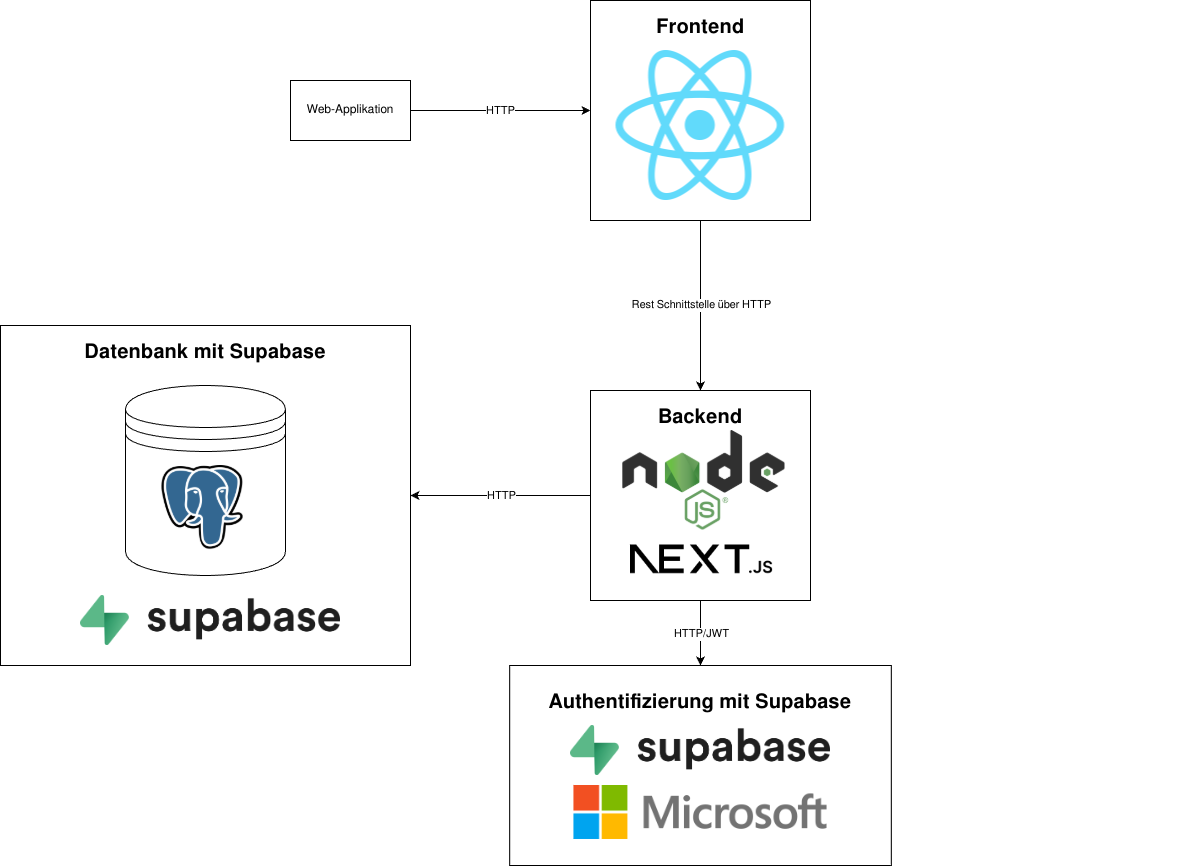
\includegraphics[width=1\textwidth]{Abbildungen/Systemarchitektur.png}
  \caption{Systemarchitektur}
  \label{fig:systemarchitektur}
\end{figure}
\newpage
\section{Literaturverzeichnis}
\end{document}
